\chapter{Contribuição}\label{meto}

A contribuição dessa pesquisa é de cunho metodológico-prático.
Do ponto de vista metodológico pela aplicação do processo CRISP-DM, usado para construir o modelo preditivo; do ponto de vista prático 
pela proposição de um modelo que integre predição à API de mapas de posicionamento global, fornecendo informação suficiente a um gestor para decidir quando 
e por onde enviar uma frota de caminhões por determinada rodovia que apresente retenções crescentes de logística de cargas. 

As soluções disponíveis que existem tais como; Google Maps, Waze e outros dessa natureza somente exibem informações momentâneas, produzidas e compartilhadas pelos utilizadores 
dos aplicativos ou por informações provindas de GPS, contudo não analisam dados históricos dessas rodovias nem fazem predições sobre o seu comportamento.

Outra contribuição dessa pesquisa é a proposição de um arco cibernético construído com a API de redes sociais.
Os ``feeds'' de notícias das redes sociais como o Twitter permitem analisar o contexto das rodovias com defasagem temporal muito pequena.
Os utilizadores dessas redes sociais contribuem com muita informação relevante como por exemplo o anúncio de uma paralisação que ocorrerá 
daqui a uma semana, a PRF de Pernambuco é outro contribuidor permanente; com seu canal no Twitter: @PRF191PE fornece diariamente informação das rodovias 
além de dados estatísticos. 

A monitoração de redes sociais é feita por Mineração de dados em textos, em que são verificas palavras chaves como: protestos, acidentes e outras.
Uma vez capturadas e tratadas, as informações desses ``feeds'' são direcionadas à um banco de dados onde será possível confrontar com o 
modelo preditivo aumentando o nível de confiança, por exemplo: no trecho da Br 101, na altura do km 5, no Município de Goiana alguém publicou
que a comunidade que mora no entorno dessa localidade fará um protesto daqui a dois dias devido ao acidente ocorrido ou a PRF publicou que o km 80
da Br 232, na altura do Município de Gravatá será interditada amanhã, por 2h, para remoção/explosão de rochas. 
Essas informações, por serem a posteriori às predições, podem aumentar o nível de confiança do utilizador e dentro de um universo temporal 
mais restrito servir de comprovação do modelo proposto.
As informações de redes sociais, armazenadas em um banco de dados, poderão servir futuramente para novas predições.

\section{Plano geral da metodologia}

A metodologia utilizada nessa pesquisa contempla um plano em três etapas, cada uma dividida em fases atinentes.
A primeira etapa da nossa metodologia completam o ciclo do processo CRISP-DM, onde está o modelo preditivo e 
a descoberta de conhecimento sobre o comportamento das rodovias. O descoberta de conhecimento sobre esses comportamento 
nas rodovias tem a ver com o ``modus operandi'' dos utilizadores, sobre possíveis erros de traçados e outros que possam
ser identificados pelos algoritmos de mineração empregados no processo.

A priori foram escolhidos algoritmos com algumas características especiais, tais como; robustez, tolerância à faltas (missing data),
aprendizagem taxa de aprendizagem, e facilidade de interpretação dos dados processados. 
No quesito robustez, tolerância à faltas e taxa de aprendizagem as redes neurais artificiais (RNA), com uma 
topologia relativamente grande destacam-se pela capacidade de generalização, contudo como todos modelos estatísticos pode ocorrer 
superadaptação (overfitting), segundo RUSSEL E NORVIG (2004)  \footnote{Foi observado que redes neurais muito grandes \textit{generalizam} bem, 
\textit{desde que os pesos sejam mantidos pequenos}. Essa restrição mantém os valores de ativação na região 
\textit{linear} da função sigmóide g(x) onde x é próximo de zero. Por sua vez isso faz com que a rede se comporte 
como uma função linear, com um número muito menor de parâmetros.} o ``overfitting''
 ocorre quando o número atributos é grande.

A extrapolação do modelo preditivo ocorre quando este se integra a um estrutura dinâmica a serem exibidas em mapas vetoriais, 
dado um espaço temporal pré-determinado por um agente; o utilizador. 
Através de APIs os mapas vetoriais permitem a geolocalização dos pontos classificados ou os pontos onde haverá grande número de 
retenções, conhecido no meio da logística de cargas como \textbf{gargalo}.
A API do Google-Maps é o ``front end'', foi escolhida por permitir maior pela portabilidade e simplicidade para integração da estrutura
dinâmica com a preditiva.

Para a integração às redes sociais, foi escolhida a API do Twitter. Esta ``interface'' é simples de ser configurada e gerar poucos dados; 
o utilizador tem que ser eficaz ao gerar suas postagem em um espaço de 140 caracteres, isso facilita a forma como os dados são
extraídos pela quantidade diminuta deles, bem como a quantidade conexões à Internet, contudo está rede social tem uma crescente quantidade
de postagens no formato imagens, isso dificulta a mineração em textos.
A API do Twitter tem a finalidade de integrar o modelo dinâmica dos mapas vetoriais às redes sociais. 
Esta ``interface'' é responsável por fornecer ``input'' à terceira etapa, servindo de ``busca local'' das informações mais recentes das 
redes sociais, relativas à trechos das rodovias; os ``feeds'' do Twitter (ou twetts) fornecem dados que serão minerados e interpretados à posteriori.

A figura a seguir ilustra essa metodologia descrita graficamente, onde as três etapas identificadas e são representadas por retângulos.

\pagebreak

\begin{figure}[ht]
\centering
\caption{Etapas da metodologia geral}
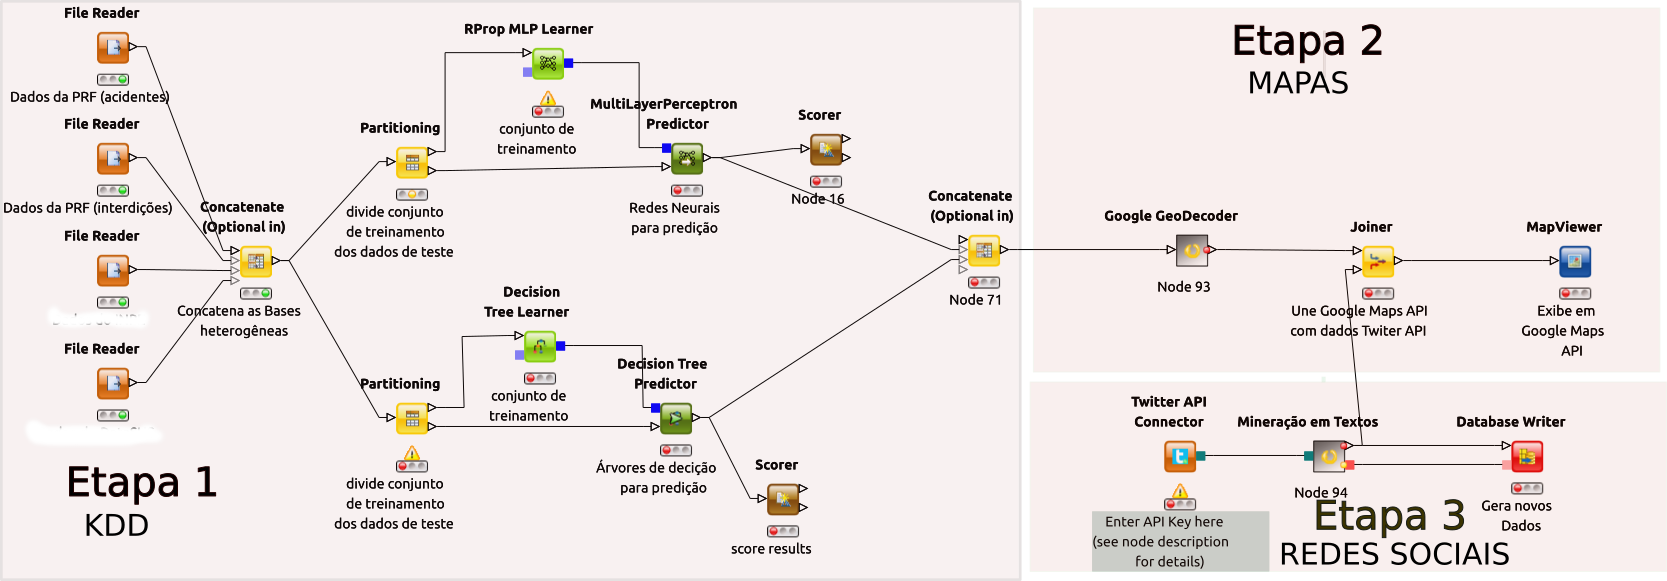
\includegraphics[width=170mm, height=85mm]{Figuras/Cronograma/metodologia.png}\\
\tiny Fonte: autor
\end{figure}

A \textbf{etapa 1} contempla a fases da coleta das bases de dados históricas, preparação dos dados e construção das variáveis do modelo preditivo.
  \begin{enumerate}
    \item O modelo preditivo integra várias bases de dados, tais como: Polícia Rodoviária Federal -- PRF, Batalhão de Polícia de Transito -- BPRv e dados históricos 
	   do Instituto de Pesquisas Espaciais -- INPE ou dos dados de precipitações pluviométricas do ``European Centre for Medium-Range Weather -- ECMWF.
 
    \item Algumas dessas informações também estão disponíveis em base de dados abertas, como sugere o Portal da Transparência, nos servidores da PRF além de outras
	  informações para complementar o sistema estão disponíveis na Internet sendo atualizadas pela PRF através de uma API aberta, esta pode 
	  ser configurável para se ligar ao nosso sistema.
    \item A conclusão dessa etapa ocorre com a Mineração dos dados e a extração de conhecimento.
	  Os ''outputs`` dessa etapa consiste em transformar os dados provenientes da mineração em coordenadas geográficas. 
	  As coordenadas geográficas são agrupadas a priori formando ''cluster`` de dados a serem exibidos em mapas vetoriais.\\
\end{enumerate}
  
A \textbf{segunda} etapa da metodologia contempla:
 \begin{enumerate}
    \item A malha viária representada em mapas de bases vetoriais;
    \item Um ambiente de simulação interativa que utiliza uma plataforma baseada na API do Google Maps.
  \end{enumerate}

A \textbf{terceira} e última etapa consiste em um módulo com as seguintes características:
  \begin{enumerate}
     \item Um módulo dinâmico onde são capturados ``feeds'' de redes sociais, por exemplo pelo Twitter. 
	Essa técnica faz um arco cibernético mantendo o sistema atualizado de informações.
     \item Através de um interligação a um banco de dados, esses ``feeds'' poderão ser usados para futuras predições.
  \end{enumerate}


\pagebreak


\section{Modelo preditivo}

O modelo preditivo foi construído utilizando bases de dados históricas da PRF (de acidentes e de paralisações ex: protestos) entre Janeiro de 2007 a 
Dezembro 2015. As bases de dados do Batalhão de Polícia de Rodoviária estadual -- BPRv vieram entre Janeiro/2010 a Julho/2016, cortes em ambas as bases foram 
feitos para adequar as datas. Essas bases de dados são integradas gerando um único e complexo modelo preditivo que será acoplado a estrutura dinâmica.


\subsection{Entendimento dos dados}
O segunda fase do ciclo CRISP-DM sugere uma análise para entendimento dos dados.
Na base de acidentes da PRF tentaremos traçar o perfil do condutor das BRs que atravessam o estado de Pernambuco.
Alguns gráfico do tipo histograma fornece uma análise explicativa desses dados de forma clara.
Na abcissa dos próximos gráficos estão os atributos mais relevantes das causas dos acidentes, elencamos os principais:
\begin{itemize}
 \item Condição da Pista: {Seca, Com burados, Molhada, Em obras, Com material granulado, Oleosa, Enlameada, Com gelo, Outras}
 \item Restrição de visibilidade: {Inexistente, Veículo Estacionado, Poeira/Fumaça/neblina, Vegetação, Ofuscamento, Cartazes/faixas, Placas}
 \item Traçado da via: {Reta, Curva, Cruzamento, Defeito}
 \item Tipo de veículo: {Automóvel, Caminhoneta, Motocicletas, Caminhão, Caminhão-trator, Bicicleta, Caminhonete, Ônibus, Motoneta, Micro-ônibus, Trator
 de rodas, Carroça, Caminhão-Tanque, Semi-Reboque, Utilitário, Ciclomotor, Charrete, Carro-de-mão, Quadriciclo, Trator misto, Reboque, Trator de esteiras,
 Não informado, Não se aplica, Não identificado}
\end{itemize}

%++++++++++++++++++++++++++++++++++++++++++++++++++++++++++++++++++++++++++++++++++++++++++++++

\begin{figure}[ht]
\begin{center}
\caption{Condição Pista X Num. Acidentes -- Restrição visibilidade X Num. Acidentes}
\subfigure[Condição da Pista: Seca]{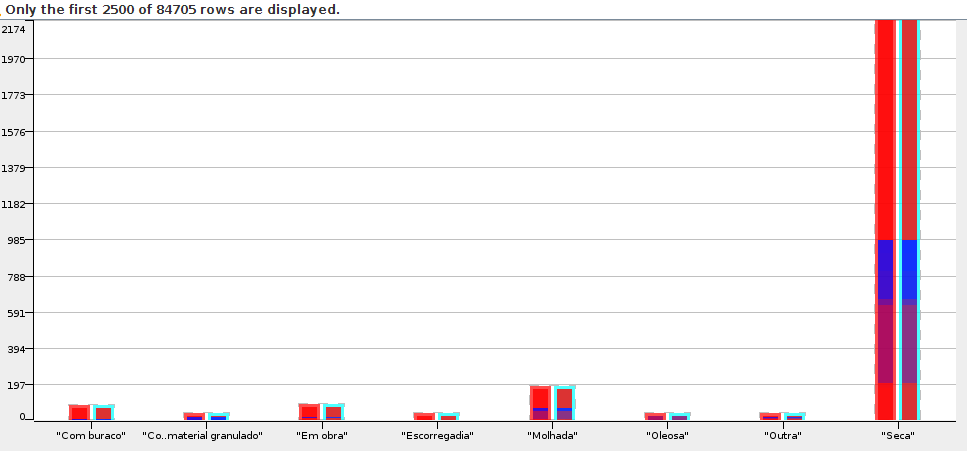
\includegraphics[width=75mm, height=48mm]{Figuras/Preprocess/CondicaoPistaXNumAcidentes.png}}
\qquad
%\caption{Restrição visibilidade X Num. Acidentes}
\subfigure[Restrição de visibilidade: Inexistente]{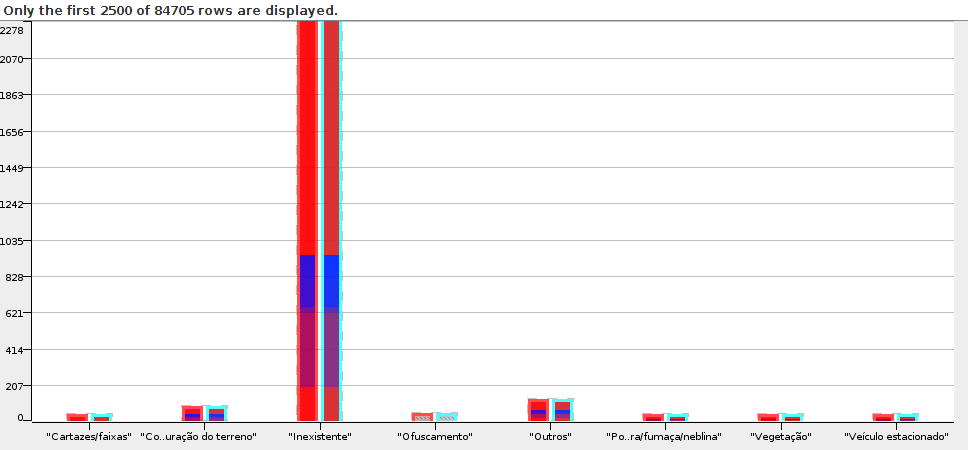
\includegraphics[width=75mm, height=48mm]{Figuras/Preprocess//RestricaoVisibilXBr.png}}\\
\tiny Fonte: autor
\end{center}
\end{figure}

A grande maioria dos acidentes ocorre com pista seca, sem restrição de visibilidade. 
A cor vermelha é referente a BR 101, a cor azul à BR 232, seguido das outras menos significativas.

\pagebreak

\begin{figure}[ht]
\begin{center}
\caption{Tipo de Veículo X Num. Acidentes}
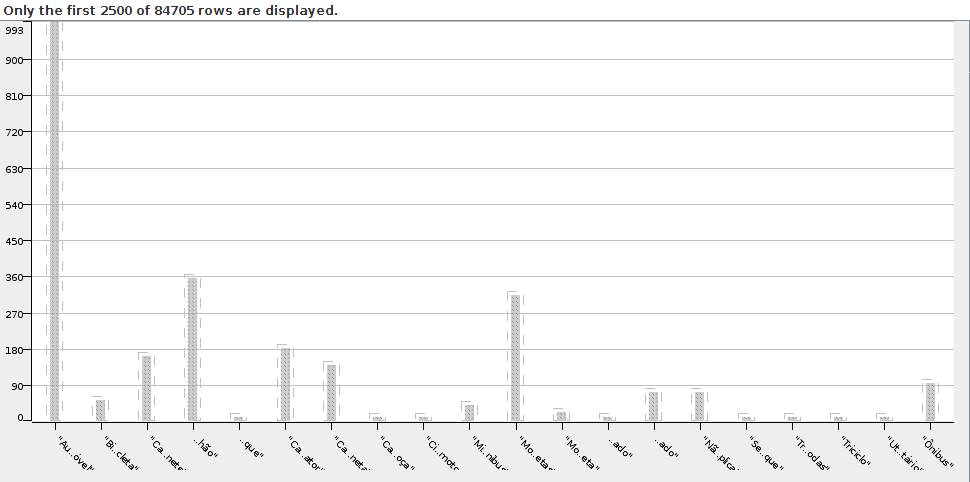
\includegraphics[width=150mm, height=80mm]{Figuras/Preprocess/TipoVeiculoXNumAciden.png}\\
\tiny Fonte: autor
\end{center}
\end{figure}

O maior número de acidentes ocorre com Automóvel de passeio, provavelmente condutores comuns, não profissionalizados.
O Caminhão é o segundo veículo que mais se envolve em acidentes, seguido das motonetas. 
Esses dados são referentes ao período entre 2007 à 2015.

\begin{figure}[ht]
\begin{center}
\caption{Traçado da via X Num. Acidentes}
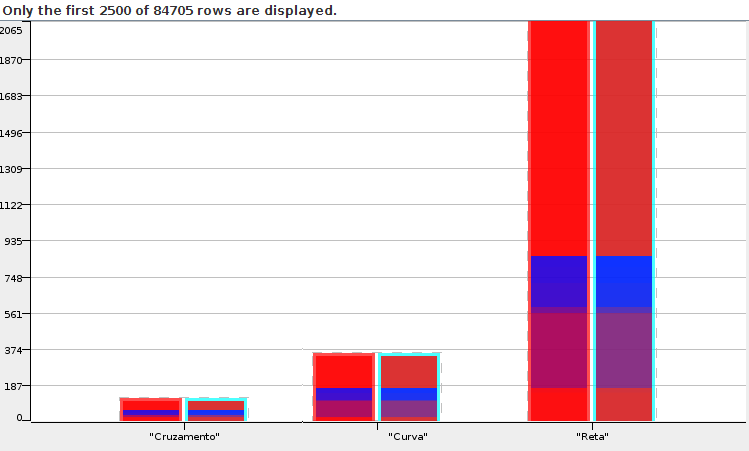
\includegraphics[width=120mm, height=70mm]{Figuras/Preprocess/TracadoViaNumAcident.png}\\
\tiny Fonte: autor
\end{center}
\end{figure}

O tipo de traçado da via não influência nas estatísticos de acidenes, pois a grande maioria dos acidentes ocorre em linha reta.
Esse comportamento do condutor nos faz crer o condutor é o responsável pelo maior número de ocorrências nas BRs.
Isso direciona nossa pesquisa para analisar e antever o comportamento do condutor, as condições da rodovia e ambientais nessa base
de dados não são fatores relevantes.

\pagebreak

\section{Reflexão sobre as tecnologias utilizadas no modelo preditivo}\label{result}

Não existe uma técnica de mineração que generalize os mais diversos ambientes preditivos, mas sim um ``pool'' 
dessas técnicas onde uma complementa outra. ((( citar )))

As técnicas preditivas tradicionais que contemplam análise de grandes massas de dados como base homogêneas.

são possíveis quando adaptadas para uma forma comparável à que
foram inicialmente concebidas, por que as variáveis em uma base de dados a priori guardam pouca relação as variáveis de outra base de dados.
neste caso essas variáveis ou são excluídas ou são transformadas a fim de ``guardarem'' um correlação com a outra base de dados. 

Na fase de transformação de dados, da primeira etapa, onde são criadas novas variáveis, a proximidade entre as
bases heterogêneas foi conseguido utilizando de regras de indução da lógica proposicional. ((( citar ))).
Nesta pesquisa, bases heterogêneas foram integralizadas num única grande conjunto de dados o ``data set''. As variáveis desse ``data set''
são consideradas variáveis independentes, foram preservadas as com maior relevância ou as que continham a maior quantidade de conhecimento
embutido.  construídas novas, nas bases onde não haviam correspondência, respeitando a lógica do negócio.\\
A tabela a seguir descreve as variáveis originais na base de dados de acidentes da PRF 


\section{Extração do conhecimento}

As técnicas como Redes Neurais Artificias (MLP) \cite{DecisaoCredito}, Árvores de decisão (CART) \cite{DataMining}, Regressão logística (MLR) 
\cite{RegrecaoLog} fornecem visão generalizada dos fatores preponderantes, levantando padrões ocultos nos dados. Esta fase é conhecida como 
Aprendizagem de Máquina (acrônimo de Machine Learning)

\begin{itemize}
 \item[a] Redes Neurais Artificias do tipo \textit{ Multi Layer Perceptron}  -- (MLP) têm capacidade de receber várias entradas ao mesmo tempo e distribuí-las de maneira organizada, além 
	  são simples de implementar e trazem resultados satisfatórios em grandes bases de dados.
 
 \item[b] Árvores de decisão do tipo \textit{ Classification and Regression Tree}  -- (CART) foi empregue por Pakgohar et al no artigo 
	  \textit{The role of human factor in incident and severity of road crashes based on the CART and LR regression a data mining approach}  para classificar acidentes 
	  com nível de acurácia próximo aos 80\%

 \item[c] Regressão logística tipo \textit{Multinomial Logistic Regression} -- (MLR) fornece a possibilidade de aprofundamento em vários níveis de busca sendo a mais apropriada, já que Regressão logística 
	  tradicional não permite aprofundamento desse tipo no espaço de busca.
\end{itemize}


\pagebreak

\section{Acoplamento com a estrutura dinâmica}

As predições feitas na primeira fase têm como ``output'' coordenadas geográficas do tipo latitude e longitude.

A estrutura dinâmica é composta por duas API's, uma disponibilizada pela Google, através do Google Maps que está atualmente na versão V3 e 
outra uma API do Twitter. A API do Google Maps proporciona uma ``leitura'' atualizada em forma de mapa no momento em que a estrutura dinâmica ``roda''.

A API do Twitter possibilita atualizar o utilizador de informações recentes, pois o modelo preditivo teve análise temporal fixada 
pelas bases de dados até 2015, portanto o fluxo decisório da predição é baseado até esse período, contudo o objetivo desta API é fazer 
um Arco Cibernético das informações, retroalimentando com dados recentes um banco de dados de redes sociais, isso permite um visualização 
instantânea do ambiente como um todo.





\begin{figure}[ht]
\centering
\caption{Etapas da metodologia}
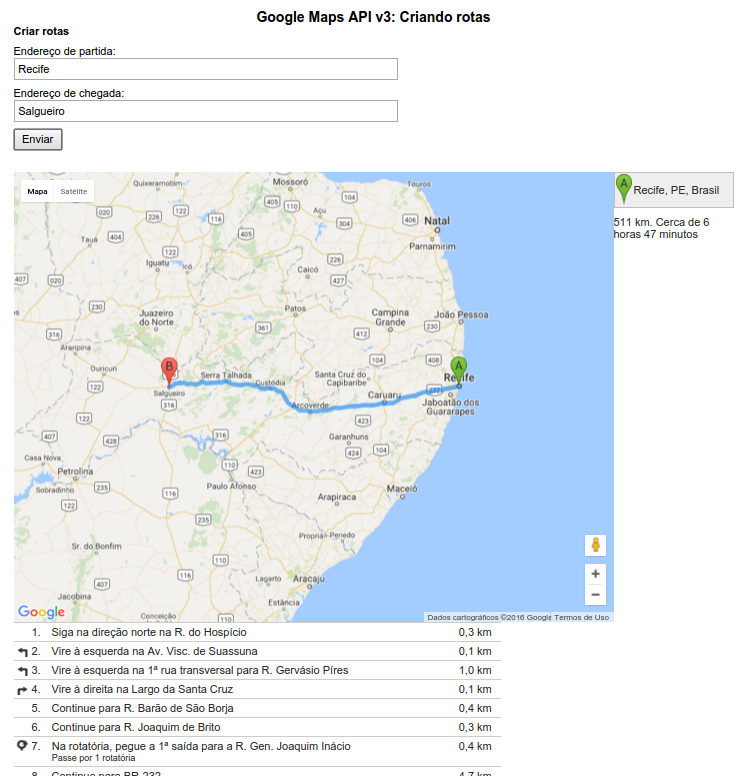
\includegraphics[width=150mm, height=130mm]{Figuras/Cronograma/GoogleMaps.png}
\end{figure}